\chapter{مقدمه‌ای بر احتمالات}
\label{ch1}
در این فصل به بیان برخی مفاهیم مورد نیاز از احتمالات خواهیم پرداخت که در ادامه به آن نیاز خواهیم داشت.

\section{احتمال}
\label{ch1:sec2:sample_space}

در نظریه احتمال به هر روندی که بتوان آن را بی‌نهایت بار تکرار کرد و همچنین بتوان یک مجموعه خوش‌ تعریف از تمام نتایج ممکن برای آن تعریف کرد \textbf{آزمایش تصادفی} گفته می‌شود. به مجموعه تمام نتایج ممکن یک آزمایش تصادفی \textbf{فضای نمونه} گفته می‌شود. به عنوان مثال مسأله پرتاب سکه یک آزمایش تصادفی است و اگر روی سکه را با $h$ و پشت سکه را با $t$ نمایش دهیم، فضای نمونه آن $\Omega = \{h,t\}$ است یا برای آزمایش تصادفی پرتاب تاس فضای نمونه به شکل $\Omega = \{1,2,3,4,5,6\}$ است. معمولاً فضای نمونه را با $\Omega$ نشان می‌دهند. 

در یک آزمایش تصادفی به هر زیرمجموعه از فضای نمونه \textbf{رویداد} گفته می‌شود. اگر نتیجه آزمایش تصادفی عضوی از یک رویداد باشد می‌گوییم آن رویداد رخ داده است. به عنوان مثال اگر دو سکه را پرتاب کنیم فضای نمونه آن به شکل زیر است.
$$\Omega = \{ \{h,h\} , \{h,t\} , \{t,h\} , \{t,t\} \}$$
فرض کنید رویداد $A$ رو آمدن سکه اول باشد بنابراین مجموعه $A$ به شکل $A = \{ \{h,h\} , \{h,t\} \}$ نوشته می‌شود. فضای نمونه $\Omega$ را هم می‌توانیم یک رویداد تعبیر کنیم، رویدادی که همیشه رخ می‌دهد و به ‌آن رویداد حتمی می‌گوییم.

از این پس مجموعه $E$ را مجموعه‌ی همه‌ی رویدادهای یک آزمایش تصادفی در نظر می‌گیریم، بنابراین همه‌ی اعضای $E$ زیر مجموعه‌‌ی $\Omega$ هستند. در ریاضیات به جفت $\{\Omega,E\}$ یک فضای قابل اندازه‌گیری گفته می‌شود که $E$ در‌ واقع جبر سیگما\LTRfootnote{σ-algebra} یا میدان سیگمای فضای نمونه $\Omega$ است.

در این ادامه به معرفی تعاریف مختلف احتمال می‌پردازیم.

\textbf{تعریف کلاسیک}: طبق این تعریف احتمال $P(A)$ رویداد $A$ به صورت $P(A)=\frac{N_A}{N}$ تعریف می‌شود که $N$ تعداد همه‌ی نتایج ممکن آزمایش تصادفی و $N_A$ تعداد نتایج مطلوب برای رویداد $A$ است. این تعریف فقط زمانی درست است که هر یک از نتایج ممکن احتمال یکسانی داشته باشند. 
مثلا در مسأله پرتاب تاس احتمال زوج آمدن تاس برابر با $\frac{3}{6}$ است که با این فرض به دست آمده که آمدن هر وجه تاس احتمال یکسانی دارد. 
 تعریف کلاسیک احتمال تاکنون با انتقادهای زیادی روبرو شده است به عنوان مثال فرض برابر بودن احتمال نتایج باعث سخت شدن تعیین $N$ و $N_A$ می‌شود. همچنین استفاده از این تعریف به مسائل خاصی محدود است.\cite{ross_first_2014}

\textbf{تعریف فرکانس نسبی}\LTRfootnote{Relative frequency}: در این تعریف احتمال رویداد $A$ از رابطه‌ی زیر به‌دست می‌آید.

\begin{equation}        
    \lim_{n\to\infty} \frac{n_a}{n}
    \label{eq1:rel_freq}
\end{equation}
در رابطه بالا $n$ تعداد کل آزمایش‌ها و $n_a$ تعداد دفعاتی است که رویداد $A$ رخ داده است. ایراد این تعریف این است که در آزمایش‌های فیزیکی عددهای $n_a$ و $n$ ممکن است خیلی بزرگ باشد اما هیچ‌گاه بی‌نهایت نیست. بنابراین در واقعیت نمی‌توان از آزمایش حد \ref{eq1:rel_freq} را محاسبه کرد و تنها می‌توانیم فرض کنیم که نسبت $\frac{n_A}{n}$ برابر حد \ref{eq1:rel_freq} است.

\textbf{اصول موضوعه احتمال}: این اصول موضوعه که با نام \textbf{اصول کولموگروف} \LTRfootnote{Kolmogorov axioms} نیز شناخته می‌شوند شامل سه اصل زیر هستند.

۱) احتمال رویداد $A$ عددی مثبت است که به رویداد $A$ نسبت داده می‌شود.
\begin{equation}
    P(A) \geq 0
    \label{eq2:axiom1}
\end{equation}
۲) به رویدادی که در هر بار انجام آزمایش رخ بدهد رویداد قطعی گفته می‌شود. اگر $S$ یک رویداد قطعی باشد احتمال این رویداد برابر ۱ است.
\begin{equation}
    P(S) = 1
    \label{eq3:axiom2}
\end{equation}
۳) اگر رویداد A و B دو رویداد ناسازگار باشند به این معنی که اشتراک آن‌ها مجموعه‌ی تهی است. داریم:
\begin{equation}
    P(A\cup B) = P(A) + P(B)
    \label{eq4:axiom3}
\end{equation}

اصول موضوعه احتمال به عنوان یک تعریف تئوری به دو تعریف دیگر ترجیح داده می‌شوند هرچند تعریف فرکانس نسبی برای کاربردهای احتمال در مسائل واقعی ضروری است. در‌ واقع  تعریف فرکانس نسبی احتمال $P(A)$ را به دفعات مشاهده یک رویداد مرتبط می‌سازد.\cite{papoulis_probability_2009}

سه مفهوم فضای نمونه، رویداد و احتمال در کنار هم، فضایی را تشکیل می‌دهند که به آن فضای احتمال گفته می‌شود. فضای احتمال در ریاضی به شکل $\{\Omega,E,P\}$ نوشته می‌شود. در ریاضی به جفت $\{\Omega,E\}$ یک فضای قابل اندازه‌گیری\LTRfootnote{Measurable space} گفته می‌شود و در ریاضیات می‌توان برای یک فضای قابل اندازه‌گیری یک سنجه تعریف کرد که طبق تعریف، سنجه به هر عضو از $E$ که همان رویدادها هستند یک عدد نسبت می‌دهد. سنجه‌ای که از اصول موضوعه احتمال پیروی کند را احتمال می‌گوییم و آن را $P$ نشان می‌دهیم.

\section{احتمال توأم و شرطی}
\label{ch1:sec4:j_cond_prob}

در احتمالات اگر بخواهیم دو یا چند رویداد را به صورت مشترک بررسی کنیم باید از مفهومی به نام احتمال توأم\LTRfootnote{Joint probability} استفاده کنیم. ممکن است این رویداد‌ها مربوط به آزمایش‌های تصادفی متفاوتی باشند اما به شکلی به هم وابسته‌اند. مثلا در بسیاری از موارد علاقه‌مند هستیم که احتمال رخ دادن دو یا چند رویداد را که به هم وابسته هستند به صورت همزمان بررسی کنیم که برای این کار باید از احتمال توأم استفاده کنیم.

تعریف احتمال توأم به شکل زیر است که $A_i$ها رویدادهایی هستند که ممکن است متعلق به ‌آزمایش‌های تصادفی متفاوتی باشند.
\begin{equation}
    P(A_1,A_2,A_3,\dotsc A_n) = P(A_1\cap A_2 \cap\dotsc A_n) 
    \label{eq5:cond_prob}
\end{equation}

به عنوان مثالی برای استفاده از احتمال توأم فرض کنید رویداد $A$ زوج آمدن یک تاس و رویداد $B$ عددی بزرگ‌تر از ۳ آمدن آن تاس باشد. بنابراین رویداد $A =\{2,4,6\}$ و رویداد $B = \{4,5,6\}$ و اشتراک این دو برابر با $A\cap B=\{4,6\}$ است. بنابراین احتمال توأم $A$ و $B$، احتمال ۴ یا ۶ آمدن تاس را بیان می‌کند. اگر دو رویداد به طور مشترک رخ ندهند یعنی اشتراکی با هم ندارند و بنابراین احتمال توأم آن‌ها صفر است.

احتمال شرطی\LTRfootnote{Conditional probability} مفهوم دیگری است که بیان کننده احتمال رخ دادن یک یا چند رویداد به شرطی است که یک یا چند رویداد دیگر رخ داده باشند یا بتوانیم فرض کنیم که رخ داده‌اند. احتمال شرطی رویدادهای $A_1, A_2,\dotsc ,A_n$ به شرط رویدادهای $B_1, B_2, \dotsc , B_m$ را با $P(A_1, A_2, \dotsc A_n \mid B_1,B_2,\dotsc B_m)$ نشان می‌دهند.

احتمال شرطی نیز مانند احتمال توأم برای بررسی رویدادهایی است که به نوعی به هم وابسته‌اند مثلاً فرض کنید در یک روز آفتابی  احتمال رخ دادن یک تصادف رانندگی در یک خیابان برابر ۰٫۰۵ و در یک روز بارانی برابر با ۰٫۱۵ باشد. در هر دو حالت، احتمال رخ دادن تصادف مورد نظر ما است، اما این احتمال وابسته به رویداد دیگری است که در اینجا شرایط آب و هوا است.

طبق تعریف کولموگروف رابطه‌ی احتمال شرطی و احتمال توأم به شکل زیر تعریف می‌شود.
\begin{equation}
    P(A \mid B) = \frac{P(A,B)}{P(B)}
    \label{cond_prob_j}
\end{equation}
اگر رابطه بالا را در P(B) ضرب کنیم داریم:
\begin{equation}
    P(A,B)=P(B)P(A \mid B)
    \label{j_prob_cond}
\end{equation}
به عبارت دیگر رابطه بالا بیان می‌کند که احتمال اینکه $A$ و $B$ هر دو رخ بدهند برابر است با احتمال رخ دادن $B$ ضرب در احتمال رخ دادن $A$ به شرطی که $B$ رخ داده باشد. شکل کلی رابطه \ref{j_prob_cond} به صورت زیر است که به آن قانون ضرب هم گفته می‌شود.
\begin{equation}
    P(A_1\cap A_2 \cap \dotsc A_n) = P(A_1)P(A_2 \mid A_1)P(A_3 \mid A_1,A_2) \dotsc P(A_n \mid A_1 \dotsc A_{n-1})
    \label{eq8:mult_rule}
\end{equation}

حالت خاصی وجود دارد که دو رویداد، مثلاً $A$ و $B$ به هم وابسته نیستند و اصطلاحاً به آن‌ها دو رویداد مستقل گفته می‌شود، در این صورت احتمال توأم آن‌ها به صورت ضرب احتمال تک تک رویدادها نوشته می‌شود.
\begin{equation}
    P(A,B) = P(A \cap B) = P(A)P(B)
    \label{eq9:independence}
\end{equation}
رابطه بالا در‌واقع تعریف دو رویداد مستقل نیز هست یعنی اگر رابطه بالا را بتوان برای دو رویداد نوشت آن دو رویداد حتما مستقل از هم هستند. اگر رابطه \ref{eq9:independence} را در رابطه \ref{cond_prob_j} جایگذاری کنیم، داریم
$$P(A \mid B) = \frac{P(A)P(B)}{P(B)} = P(A)$$
که بیانگر این است که رویداد $A$ وابستگی به $B$ ندارد. واضح است که این رابطه را برای وابستگی رویداد $‌B$ به $A$ نیز می‌توان نوشت.\cite{taylor_introduction_1998}


\section{متغیر تصادفی}
\label{ch1:sec5:random_variable}

همان‌طور که در بخش \ref{ch1:sec2:sample_space} گفته شد هر آزمایش تصادفی دارای یک فضای نمونه است که مجموعه‌ای از تمام نتایج ممکن آزمایش تصادفی است. متغیر تصادفی عددی است که به هر یک از نتایج یک آزمایش تصادفی نسبت می‌دهیم به عنوان مثال در یک آزمایش پرتاب سکه می‌توانیم متغیر تصادفی را به این شکل تعریف کنیم که اگر روی سکه آمد مقدار متغیر برابر ۱ و اگر پشت سکه آمد مقدار متغیر برابر صفر باشد.
به عبارت دیگر متغیر تصادفی تابعی است که دامنه‌ی آن فضای نمونه آزمایش تصادفی و برد آن یک فضای قابل اندازه‌گیری است. اگر $\mathbf{x}$ متغیر تصادفی و $r$ نتیجه‌ی آزمایش تصادفی باشد می‌توان گفت:
$$
\begin{array}{l}
    \mathbf{x}:\Omega \rightarrow S \\
    \mathbf{x}(r\in \Omega) = X \in S
\end{array}
$$
در تعریف بالا $S$ یک فضای قابل اندازی‌گیری است که در بسیاری موارد $S=\mathbb{R}$ است. اگر $X \in S$ باشد، احتمال اینکه $\mathbf{x}=X$ بشود به شکل زیر تعریف می‌شود.
$$
P(X \in S) = P(\{ r \in \Omega \mid \mathbf{x}(r) = X \})
$$
در برخی از شرایط نیاز است که بدانیم احتمال اینکه متغیر تصادفی $\mathbf{x}$ مقداری کمتر از عدد $X$ بگیرد چقدر است، یا احتمال اینکه $\mathbf{x}$ بین $X_1$ و $X_2$ باشد چقدر است. برای یافتن این احتمال باید نتایجی را یافت که متغیر تصادفی $\mathbf{x}$ برای آن‌ها بین $X_1$ و $X_2$ باشد، احتمال این رویداد همان احتمالی است که $\mathbf{x}$ بین $X_1$ و $X_2$ باشد. به عبارت دیگر:
$$
P(X_1 \leq \mathbf{x} \leq X_2) = P(\{ r \in \Omega  \mid X_1 \leq  \mathbf{x}(r) \leq X_2 \})
$$

\subsection{متغیر تصادفی پیوسته}
\label{ch1:sec6}
تا اینجا تنها متغیرهای تصادفی با فضای نمونه گسسته را بررسی کرده‌ایم و همان‌طور که گفته شد  $P$ تابعی است که احتمال رویدادها را مشخص می‌کند معمولاً به $P$ \textbf{تابع توزیع احتمال}\LTRfootnote{Probability distribution function} گفته می‌شود، اما متغیرهای تصادفی پیوسته نیز وجود دارند که فضای نمونه آن‌ها ناشمارا است به عبارت دیگر مقادیر یک متغیر تصادفی پیوسته می‌تواند هر مقداری از یک بازه‌ی پیوسته باشد. در این شرایط چون فضای نمونه یک بازه پیوسته است و در نتیجه تعداد ناشمارایی رویداد خواهیم داشت باید احتمال رویدادها را به شکل دیگری بررسی کنیم. 

 فرض کنید $f( x )$ یک تابع مثبت باشد که در بازه  $(-\infty, +\infty)$ تعریف شده باشد. همچنین احتمال اینکه مقدار $X$ عضوی از مجموعه $A$ باشد را بتوان با انتگرال $f$ روی مجموعه $A$ به دست آورد، در این صورت $x$ را یک متغیر تصادفی پیوسته می‌گوییم. به عبارت دیگر 
 \begin{equation}
    P\{x \in A\}=\int_{A} f(x) d x
    \label{density1}
\end{equation}
تابع $f$ را \textbf{تابع چگالی احتمال}\LTRfootnote{Probability density function} متغیر تصادفی $x$ گوییم. از آنجایی که $x$ حتماً باید مقدار داشته باشد، بنابراین
\begin{equation}    
    P\{x \in(-\infty, \infty)\}=\int_{-\infty}^{\infty} f(x) d x=1
    \label{p_normalization}
\end{equation}
که بیانگر آن است که جمع روی احتمال همه نتایج ممکن برابر با یک است، به رابطه بالا شرط نرمال بودن می‌گویند که شرطی لازم برای هر توزیع احتمال است.

اگر در رابطه \ref{density1} مجموعه‌ $A$ می‌تواند بازه $[a,b]$ باشد بنابراین
 \begin{equation}
    P\{a \leq x \leq b\}=\int_{a}^{b} f(x) d x
    \label{density2}
\end{equation}
که احتمال اینکه $x$ مقداری بین $a$ تا $b$ داشته باشد را بیان می‌کند. در رابطه \ref{density2} اگر $a=b$ داریم
$$
    P\{x=a\}=\int_{a}^{a} f(x) d x=0
$$
که به این معنی است که احتمال اینکه متغیر تصادفی یک مقدار معین داشته باشد صفر است. از آنجایی که انتگرال بالا به معنی احتمال است بنابراین  تابع چگالی احتمال یک تابع بی بعد مانند توزیع احتمال نیست و بعدی عکس بعد متغیر تصادفی دارد.

کمیت مهم دیگر \textbf{تابع توزیع تجمعی}\LTRfootnote{Cumulative distribution function} است که آن را با $F(y)$ نشان می‌دهیم و رابطه آن با تابع چگالی احتمال به شکل زیر است
\begin{equation}
    F(y)=P\{x \in(-\infty, a]\}=\int_{-\infty}^{y} f(x) d x
    \label{cumulative1}
\end{equation}
اگر از دو طرف رابطه بالا مشتق بگیریم داریم
\begin{equation}
    \frac{d}{d y} F(y)=f(y)
    \label{cumulative_density}
\end{equation}
که نشان دهنده این است که تابع چگالی احتمال مشتق توزیع تجمعی است.

از رابطه \ref{density2} می‌توانیم به تفسیر دیگری از چگالی احتمال برسیم، اگر بازه انتگرال $( a-\frac{\varepsilon}{2}, a+\frac{\varepsilon}{2} )$ باشد و $\varepsilon$ مقدار کوچکی داشته باشد، با استفاده از بسط تیلور می‌توانیم بنویسیم:
\begin{equation}
    P\left\{a-\frac{\varepsilon}{2} \leq x \leq a+\frac{\varepsilon}{2}\right\}=\int_{a-\varepsilon / 2}^{a+\varepsilon / 2} f(x) d x \approx \varepsilon f(a)
\end{equation}
به عبارت دیگر احتمال اینکه   $x$ مقداری در بازه‌ای به طول $\varepsilon$ اطراف $a$ داشته باشد تقریباً برابر $\varepsilon f(a)$ است، مشخص است که $f(a)$ معیاری است از احتمال اینکه متغیر تصادفی در نزدیکی $a$ باشد.

یکی از روابط مهم در خصوص توزیع و چگالی احتمال، رابطه توزیع مارجینال\LTRfootnote{Marginal distribution} است که به شکل زیر بیان می‌شود.
\begin{equation}
    \begin{array}{ll}
        P(x_1, \ldots, x_{i-1})=\sum_{i} P(x_{1}, \ldots, x_{i}) & \qquad \qquad {\text{برای متغیر تصادفی گسسته}} \\
        f(x_1, \ldots, x_{n-1})=\int_{-\infty}^{\infty} f(x_{1}, \ldots, x_{n}) d x_{n} & { \qquad \qquad \text {برای متغیر تصادفی پیوسته}}
\end{array}
    \label{marginalization}
\end{equation}
این رابطه در عین سادگی رابطه‌ای مهم در احتمالات است، در فصل بعد از این رابطه استفاده خواهیم کرد.

\section{خواص توزیع احتمال}
\label{ch1:sec7}

در این بخش برخی از کمیت‌ها مانند مقادیر چشم‌داشتی و انباشتک‌ها که می‌توان از تابع توزیع احتمال به دست آورد خواهیم پرداخت.

\subsection{مقادیر چشم‌داشتی و ممان}

یکی از مهم‌تررین مفاهیم در نظریه احتمالات، مقدار چشم‌داشتی یک متغیر تصادفی است. برای یک متغیر تصادفی گسسته مقدار چشم‌داشتی یا همان میانگین یک متغیر تصادفی از رابطه زیر به دست می‌آید و آن را با  $<x>$ نشان می‌دهند.
\begin{equation}
<x>=\left\{\begin{array}{ll}{\sum_{i} x_{i} P(x_{i})} & \qquad \qquad {\text{برای متغیر تصادفی گسسته}} \\ 
{\int x f(x) d x} & { \qquad \qquad \text {برای متغیر تصادفی پیوسته}}\end{array}\right.
\label{mean}
\end{equation}
به عبارت دیگر چشم‌داشتی $x$ یک میانگین وزن دار از تمام مقادیر ممکن $x$ است. مثلاً در شرایطی که توزیع احتمال یکنواخت است به این معنی که احتمال همه نتایج با یکدیگر یکسان است مقدار چشم‌داشتی همان رابطه معمولی برای میانگین است.

در بسیاری از مواقع نیاز است که چشم‌داشتی تابعی مثلا $g(x)$ از یک متغیر تصادفی را بدانیم در این صورت به شکل زیر این مقادیر نیز به دست می‌آیند.
\begin{equation}
    <g(x)>=\left\{\begin{array}{ll}{\sum_{i} g(x_{i}) P(x_{i})} & \qquad \qquad {\text{برای متغیر تصادفی گسسته}} \\ 
    {\int g(x)  f(x) d x} & { \qquad \qquad \text {برای متغیر تصادفی پیوسته}}\end{array}\right.
    \label{expect_func}
\end{equation}
به چشم‌داشتی توابع به شکل $g(x) = x^k$ که $k=0,1,\dotsc,n$ است،  ممان\LTRfootnote{Moment} $k$اٌم گفته می‌شود که از مهمترین مقادیر چشم‌داشتی در نظریه احتمالات هستند. ممان صفرم یعنی زمانی که $k=0$ باشد معادله \ref{expect_func} تبدیل به معادله \ref{p_normalization} می‌شود که به معنی جمع احتمال همه نتایج ممکن است و به دلیل نرمال بودن توزیع احتمال برابر با یک است. ممان اول نیز همان رابطه \ref{mean} است.  

\subsection{توابع مولد ممان}
همان‌طور که در بخش قبل گفته شد ممان‌ها کمیت‌های مهمی هستند، یک توزیع احتمال با استفاده از ممان‌هایش توصیف می‌شود. در این بخش تابعی را معرفی می‌کنیم که با استفاده از آن می‌توان ممان‌های توزیع احتمال یک متغیر تصادفی را به دست آورد که به آن تابع مولد ممان\LTRfootnote{Moment generating function} گفته می‌شود. با توجه به بخش قبل برای متغیر تصادفی $x$ اگر $g(x) = e^{tx}$ که $t$ یک عدد حقیقی است به تابع زیر تابع مولد ممان گفته می‌شود.
\begin{equation}
M_{x}(t)=<e^{t x}>=\left\{\begin{array}{ll}{\sum_{i} e^{t x_{i}} P(x_{i})} & \qquad \qquad {\text { برای متغیر تصادفی گسسته }} \\ 
{\int e^{t x} f(x) d x} & \qquad \qquad {\text { برای متغیر تصادفی پیوسته }}\end{array}\right.
\end{equation}
از آنجایی که به ازای $t=0$ تابع مولد ممان مقداری برابر با یک دارد پس در $t=0$ این تابع همیشه با معنی است، به ازای بقیه مقادیر $t$ به شرطی که $x$ متناهی باشد این تابع با معنی است.
همان‌طور که از نام تابع مولد ممان مشخص است از این تابع می‌توان برای به دست آوردن ممان‌های یک توزیع احتمال استفاده کرد، برای این کار باید $M_{x}(x)$ را حول $t=0$ بسط دهیم. داریم

\begin{equation}
\begin{aligned} <e^{t x}> &=<1+t x+\frac{t^{2} x^{2}}{2 !}+\cdots> =1+E<x> t+E<x^{2}> \frac{t^{2}}{2 !}+\cdots \end{aligned}
\label{mfg_expansion}
\end{equation}
با توجه به بسط تابع مولد ممان می‌توان این‌طور برداشت کرد که ممان‌های یک توزیع احتمال با مشتق تابع مولد ممان در $t=0$ برابر است. یعنی
\begin{equation}
    <x^{n}>=\left.\frac{d^{n} M_{x}(t)}{d t^{n}}\right|_{t=0}
\end{equation}
به این صورت با مشتق گیری از تابع مولد ممان می‌توان ممان‌های یک توزیع را به دست آورد.
نکته مهم این است که اگر تابع مولد ممان دو متغیر تصادفی با هم برابر باشد بنابراین توزیع احتمال این دو متغیر تصادفی نیز با یکدیگر برابر است.

\subsection{تابع مشخصه}
تعریف تابع مشخصه\LTRfootnote{Characteristic function} به شکل زیر است.
\begin{equation}
C_{x}(t)=<e^{i t x}>=\left\{\begin{array}{ll}{\sum_{j} e^{i t x_{j}} P(x_{j})} & \qquad \qquad {\text { برای متغیر تصادفی گسسته}} \\ 
{\int e^{i x} f(x) d x} & \qquad \qquad {\text { برای متغیر تصادفی پیوسته }}\end{array}\right.
\label{charach_func}
\end{equation}
تابع مشخصه یک متغیر تصادفی در‌واقع به نوعی همان تابع مولد ممان است درواقع $M_{x}(it)$ دقیقاً همان تابع مشخصه است. همان‌طور که تعریف تابع مشخصه و تابع مولد ممان مشابه یکدیگر است موارد استفاده و کاربردهای این دو نیز به یکدیگر نزدیک است. ویژگی‌های که برای تابع مولد ممان گفته شده را می‌توان با استفاده از $C_{x}(t) = M_{x}(it)$ برای تابع مشخصه به دست آورد. به عنوان مثال ممان‌های $x$ بر حسب مشتق‌های تابع مشخصه $C_{x}(t)$ را می‌توان با رابطه زیر به دست آورد.
\begin{equation}
    <x^{n}>=(-i)^{n} C_{x}^{(n)}(0) = \mu_{n}
\end{equation}
که در رابطه بالا 
$$
C_{x}^{( n )}(0) = \left. \frac{d^{n} C_{x}(t)}{d^{n} t} \right|_{t=0}
$$
این که برای توصیف یک متغیر تصادفی از تابع مولد ممان یا تابع مشخصه استفاده کنیم تا حدی یک موضوع شخصی است. اگرچه استفاده از تابع مشخصه مزایایی دارد، مهمترین آن جایگزینی تابع نمایی $e^{tx}$ در تابع مولد ممان با تابع نوسانی مختلط $e^{itx}$ در تابع مشخصه است. مزیت این جایگزینی این است که در تابع مولد ممان باید مراقب واگرا شدن این تابع باشیم اما برای تابع مشخصه به دلیل داشتن رفتار نوسانی نگرانی در این مورد وجود ندارد. علاوه بر این زمانی که $x$ یک متغیر تصادفی پیوسته است رابطه \ref{charach_func} با تبدیل فوریه تابع چگالی احتمال $f(x)$ مرتبط است. بنابراین می‌توان چگالی احتمال $f(x)$ را با استفاده از تبدیل معکوس فوریه از تابع مشخصه به دست آورد.
\begin{equation}
    f(x)=\frac{1}{2 \pi} \int_{-\infty}^{\infty} C_{x}(t) e^{-i t x} d t
\end{equation}

\subsection{تابع مولد انباشتک}
انباشتک‌ها\LTRfootnote{Cumulant} از مهمترین کمیت‌های مرتبط با یک توزیع احتمال هستند و می‌توان آن‌ها را بر حسب ممان‌های یک توزیع احتمال به دست آورد. بهترین راه برای به دست آوردن انباشتک‌ها استفاده از تابع مولد انباشتک\LTRfootnote{Cumulant generating function} است که آن را با $K_{x}(t)$ نشان می‌دهیم. طبق تعریف تابع مولد انباشتک برابر است با لگاریتم طبیعی تابع مولد ممان و اگر $K_{x}(t)$ را به صورت یک سری توانی از $t$ بسط دهیم ضریب جمله $\frac{t^k}{k!}$ انباشتک $k$اٌم تابع چگالی احتمال $f(x)$ است. یعنی
\begin{equation}
    K_{x}(t)=\ln M_{x}(t) \equiv \kappa_{1} t+\kappa_{2} \frac{t^{2}}{2 !}+\kappa_{3} \frac{t^{3}}{3 !}+\cdots
    \label{cfg_expansion}
\end{equation}
می‌توانیم انباشتک‌های یک توزیع را با مشتق گرفتن از تابع مولد انباشتک نسبت به $t$ به دست آوریم
\begin{equation}
    \frac{d K_{x}}{d t}=\frac{1}{M_{x}} \frac{d M_{x}}{d t} \Rightarrow M_{x} \frac{d K_{x}}{d t} = \frac{d M_{x}}{d t}
\end{equation}
با استفاده از \ref{mfg_expansion} و \ref{cfg_expansion} می‌توانیم بنویسیم
\begin{equation}
    (\kappa_{1}+\kappa_{2} t+\kappa_{3} \frac{t^{2}}{2 !}+\cdots)(1+\mu_{1} t+\mu_{2} \frac{t^{2}}{2 !}+\cdots)=(\mu_{1}+\mu_{2} t+\mu_{3} \frac{t^{2}}{2 !}+\cdots)
\end{equation}
با برابر قرار دادن ضرایب توان‌های $t$ در دو طرف تساوی می‌توانیم بنوسیم
$$
\begin{aligned} \mu_{1} &=\kappa_{1} \\ \mu_{2} &=\kappa_{2}+\kappa_{1} \mu_{1} \\ \mu_{3} &=\kappa_{3}+2 \kappa_{2} \mu_{1}+\kappa_{1} \mu_{2} \\ & \vdots \\ \mu_{k} &=\kappa_{k}+^{k-1} C_{1} \kappa_{k-1} \mu_{1}+\cdots+^{k-1} C_{r} \kappa_{k-r} \mu_{r}+\cdots+\kappa_{1} \mu_{k-1} \end{aligned}
$$
\begin{figure}[htb]
    \centering
    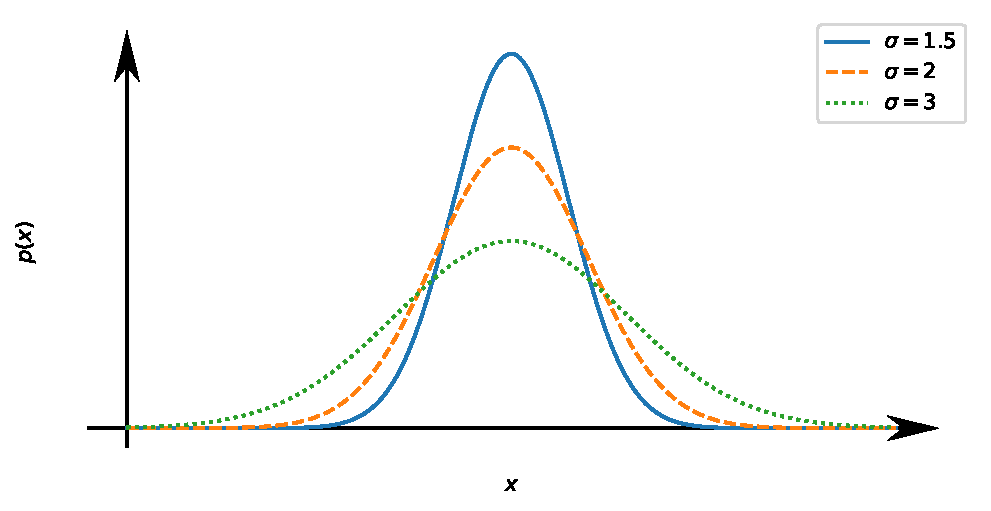
\includegraphics[width=0.8\textwidth]{images/dist_variance_effect.pdf}
    \caption{اثر انحراف معیار بر توزیع نرمال} %\label{fig:std}
    \par\medskip
\captionsetup{justification=centering}
\end{figure}
\FloatBarrier
با حل این معادلات می‌توانیم انباشتک‌ها را بر حسب ممان‌ها به دست آوریم. چهار ممان اول به صورت زیر به دست می‌آیند.
\begin{equation}
\begin{array}{l}{\kappa_{1}=\mu_{1}} \\ {\kappa_{2}=\mu_{2}-\mu_{1}^{2}=v_{2}} \\ {\kappa_{3}=\mu_{3}-3 \mu_{2} \mu_{1}+2 \mu_{1}^{3}=v_{3}} \\ {\kappa_{4}=\mu_{4}-4 \mu_{3} \mu_{1}+12 \mu_{2} \mu_{1}^{2}-3 \mu_{2}^{2}-6 \mu_{1}^{4}=v_{4}-3 v_{2}^{2}}\end{array}
\end{equation}
همان‌طور که پیداست انباشتک اول درواقع همان میانگین توزیع است. به انباشتک دوم واریانس گفته می‌شود  همچنین به مجذور واریانس نیز انحراف معیار گفته می‌شود که معمولا آن را با $\sigma$ نشان می‌دهند. واریانس معیاری از پراکندگی مقادیر متغیر تصادفی $x$ حول میانگین هستند.
انباشتک سوم چولگی نام دارد و معیاری از عدم تقارن چگالی احتمال حول میانگین است واگر چولگی برابر با صفر باشد توزیع حول میانگین تقارن کامل دارد. در شکل زیر اثر چولگی مثبت و منفی نشان داده شده است.

\begin{figure}[htb]
    \centering
    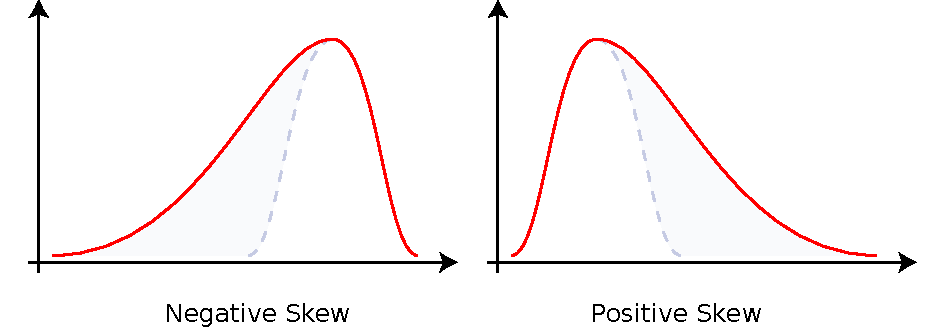
\includegraphics[width=0.8\textwidth]{images/skewness.pdf}
    \caption{اثر چولگی بر توزیع احتمال\cite{wiki:xxx}} %\label{fig:std}
    \par\medskip
\captionsetup{justification=centering}
\end{figure}
\FloatBarrier

انباشتک چهارم کشیدگی یا برجستگی نام دارد که توصیف کننده میزان مسطح بودن یا قله‌ای بودن یک توزیع احتمال است. هرچه کشیدگی یک توزیع مقدار بزرگ‌تری داشته باشد، آن توزیع قله‌ای‌تر و دنباله پهن‌تری دارد. 
% در شکل زیر اثر کشیدگی نشان داده شده است.

% \begin{figure}[htb]
%     \centering
%     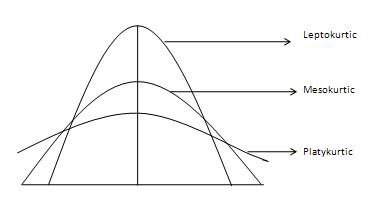
\includegraphics[scale=1]{images/kurtosis.jpeg}
%     \caption{اثر کشیدگی بر توزیع احتمال} %\label{fig:std}
%     \par\medskip
% \captionsetup{justification=centering}
% \end{figure}
% \FloatBarrier

\section{توزیع‌‌های احتمال پرکاربرد}
\label{ch1:sec8}
در این بخش به معرفی چند توزیع احتمال پرکاربرد در احتمالات می‌پردازیم.

\subsection{توزیع دو جمله‌ای}
یکی از مهمترین توزیع‌های احتمال‌ گسسته توزیع احتمال دو جمله‌ای\LTRfootnote{Binomial distribution} است. این توزیع شامل تعدادی مثلاً $n$ بار آزمایش مستقل با دو نتیجه ممکن مثلاً $A$ و $B$ است که این دو نتیجه اشتراکی با هم ندارند. به عنوان مثال این دو نتیجه می‌توانند $T$ یا $H$ آمدن سکه باشد یا موفقیت یا عدم موفقیت یک آزمایش تصادفی باشند.
فرض کنید احتمال موفقیت یک آزمایش تصادفی برابر $p$ باشد و احتمال عدم موفقیت  برابر $q = 1-p$ باشد در این صورت اگر $n$ بار آزمایش را مستقل از هم تکرار کنیم می‌توانیم متغیر تصادفی $x$ را برابر تعداد بارهایی که آزمایش موفق است تعریف کنیم. حال احتمال اینکه تعداد $x$ بار آزمایش موفق باشد و $n-x$ بار ناموفق باشد برابر است با
\begin{equation}
    \operatorname{P}(x ; n, p) =\left( \begin{array}{l}{n} \\ {x}\end{array} \right) p^{x}(1-p)^{n-x}
    \end{equation}
\begin{figure}[htb]
    \centering
    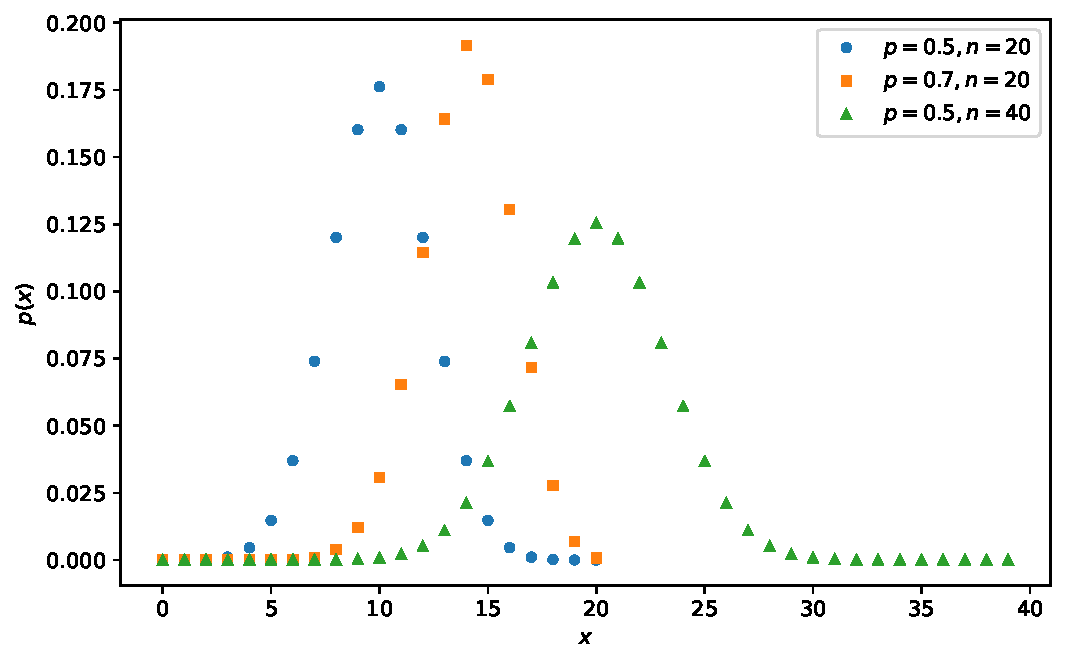
\includegraphics[width=0.9\textwidth]{images/binomial.pdf}
    \caption{چند نمونه از توزیع دو جمله‌ای} %\label{fig:std}
    \par\medskip
\captionsetup{justification=centering}
\end{figure}
\FloatBarrier

یرخی از ویژگی‌های توزیع دو جمله‌ای در جدول زیر آمده است.

\bgroup
\def\arraystretch{1.5}
\begin{table}[htb]
    \centering
    \caption{برخی از ویژگی‌های توزیع دو جمله‌ای}
    \begin{tabular}{ c c }
    \hline
     \vspace{4pt}
     میانگین & $np$ \\ \hline
     \vspace{4pt}
     واریانس & $npq$ \\ \hline
     \vspace{4pt}
     چولگی & $\frac{q-p}{\sqrt{npq}}$ \\ \hline
     \vspace{4pt}
     کشیدگی & $\frac{1-6pq}{npq}$ \\ \hline
     \vspace{4pt}
    \end{tabular}
\end{table}
\egroup
\FloatBarrier

\subsection{توزیع پواسون}
توزیع پواسون\LTRfootnote{Poisson distribution} برای شرایطی است که تعداد دفعات انجام آزمایش زیاد باشد یعنی زمانی که $n \rightarrow \infty$، مثلاً فرض کنید که مسأله مورد نظر تعداد تماس‌هایی است که در یک بازه زمانی با یک مرکز تلفن می‌شود. با در نظر گرفتن یک نرخ رخداد $\lambda$ در واحد زمان، توزیع پواسون $P(x)$ احتمال اینکه دقیقا $x$ بار رویداد در واحد زمان رخ بدهد را نشان می‌دهد.\cite{Walck1996HandbookOS}
\begin{figure}[htb]
    \centering
    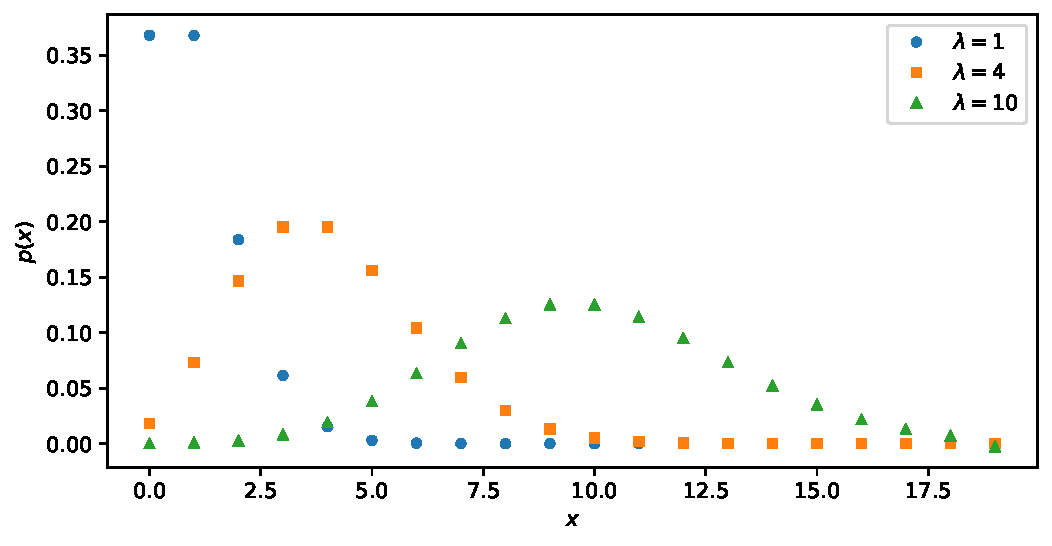
\includegraphics[width=0.6\textwidth]{images/poisson.pdf}
    \caption{چند نمونه از توزیع پواسون} %\label{fig:std}
    \par\medskip
\captionsetup{justification=centering}
\end{figure}
\FloatBarrier
توزیع پواسون در‌واقع حالت حدی توزیع دو جمله‌ای است زمانی که $n \rightarrow \infty$ و احتمال اینکه رویداد رخ بدهد نزدیک به صفر باشد یعنی $p \rightarrow 0$، به شرطی که حاصل ضرب $np$ مقداری متناهی $\lambda$ باشد. شکل ریاضی توزیع پواسون به شکل زیر است.

\begin{equation}
    f(k ; \lambda)=\operatorname{P}(x=k)=\frac{\lambda^{k} e^{-\lambda}}{k !}
\end{equation}

برخی از ویژگی‌های توزیع پواسون در ادامه آمده است.
\bgroup
\def\arraystretch{1.5}
\begin{table}[htb]
    \centering
    \caption{برخی از ویژگی‌های توزیع پواسون}
    \begin{tabular}{ c c | c c}
    \hline
    %  \vspace{4pt}
     میانگین & $\lambda$ & واریانس & $\lambda$ \\ \hline
    %  \vspace{4pt}
     چولگی & $\lambda^{-1/2}$ & کشیدگی & $\lambda^{-1}$ \\ \hline
    %  \vspace{4pt}
    \end{tabular}
\end{table}
\egroup
\FloatBarrier

\subsection{توزیع گاوسی}

توزیع گاوسی\LTRfootnote{Gaussion distribution} که به آن توزیع نرمال\LTRfootnote{Normal distribution} هم گفته می‌شود مهمترین توزیع پیوسته است. دلیل اهمیت توزیع نرمال این است که تعداد خیلی زیادی از متغیرهای تصادفی مورد مطالعه در همه زمینه‌های  علمی به طور دقیق یا تقریبی با توزیع گاوسی توصیف می‌شوند. توزیع گاوسی به شکل زیر بیان می‌شود.

\begin{equation}
    p(x) = \frac{1}{\sigma \sqrt{2 \pi}} e^{-\frac{1}{2}(\frac{x-\mu}{\sigma})^{2}}
    \label{normal_dist}
\end{equation}
در رابطه بالا $\mu$ میانگین و $\sigma$ انحراف معیار هستند و ضریب $\frac{1}{\sigma \sqrt{2 \pi}}$ را ضریب نرمال سازی می‌گویند که از شرط نرمال بودن \ref{p_normalization} به دست می‌آید.
توزیع گاوسی را نیز می‌توان یکی از حالت‌های حدی توزیع دو جمله‌ای در نظر گرفت. توزیع گاوسی در شرایطی به دست می‌آید که $n \rightarrow \infty$ و همچنین احتمال $p$ نیز مقداری متناهی داشته باشد و در نتیجه $np \rightarrow \infty$.
\begin{figure}[htb]
    \centering
    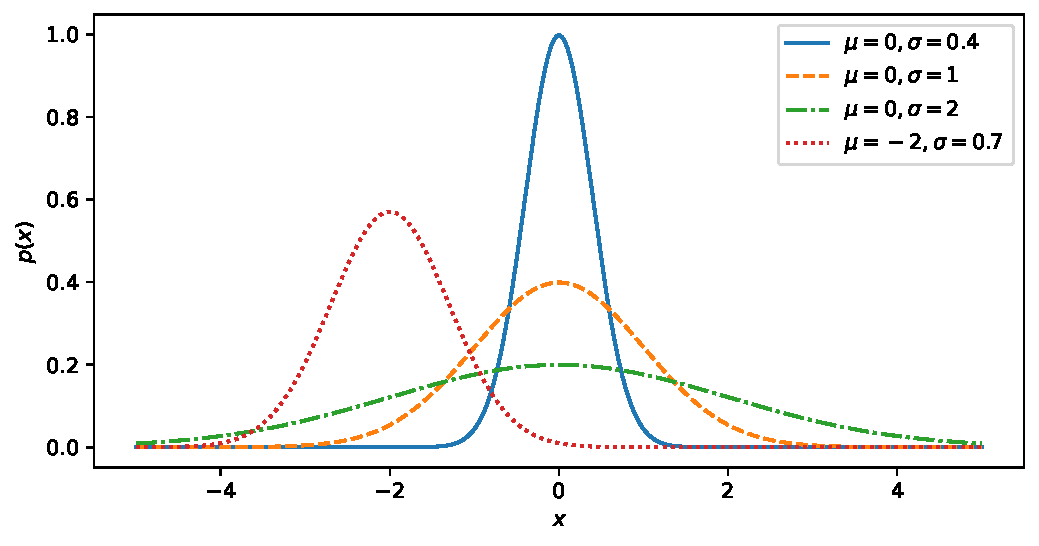
\includegraphics[width=0.9\textwidth]{images/normal.pdf}
    \caption{چند نمونه از توزیع گاوسی} %\label{fig:std}
    \par\medskip
\captionsetup{justification=centering}
\end{figure}
\FloatBarrier
حدود $\%68.2$ از اعدادی که از توزیع نرمال می‌آیند در بازه $[\mu-\sigma, \mu+\sigma]$ قرار می‌گیرند. 
 یعنی در فاصله‌ای کمتر یا برابر با انحراف معیار نسبت به میانگین قرار می‌گیرند 
و تقریبا $\%95.4$ از اعداد در بازه $[\mu-2\sigma, \mu+2\sigma]$ قرار می‌گیرند.
یکی دیگر از ویژگی‌های مهم توزیع گاوسی صفر بودن ممان‌های سوم و بالاتر است بنابراین توزیع نرمال یک توزیع متقارن حول میانگین است. 
% در جدول زیر ویژگی‌های توزیع گاوسی آمده است.
% \bgroup
% \def\arraystretch{1.5}
% \begin{table}[htb]
%     % \centering
%     \begin{tabular}{ c c }
%     \hline
%      \vspace{4pt}
%      میانگین & $\mu$ \\ \hline
%      \vspace{4pt}
%      واریانس & $\sigma^{2}$ \\ \hline
%      \vspace{4pt}
%      چولگی & $0$ \\ \hline
%      \vspace{4pt}
%      کشیدگی & $0$ \\ \hline
%      \vspace{4pt}
%     \end{tabular}
%     \caption{برخی از ویژگی‌های توزیع گاوسی}
% \end{table}
% \egroup
% \FloatBarrier

